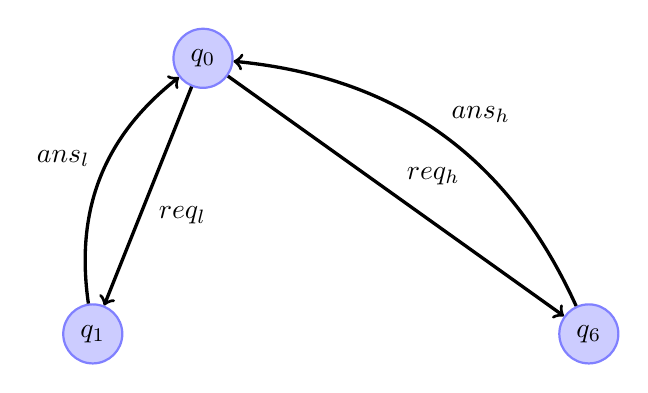
\begin{tikzpicture}[scale=0.7]
	\node 	(q0)		at	(0,5) 	[circle, thick, draw=blue!50,fill=blue!20,inner sep=0pt,minimum size=.75cm]{$q_0$};


	\node 	(q1)		at	(-2,0) 	[circle, thick, draw=blue!50,fill=blue!20,inner sep=0pt,minimum size=.75cm]{$q_1$}
		edge[<-,very thick]			node[auto,swap]{$req_l$}	(q0);

%	\node 	(q2)		at	(-4,-3) 	[circle, thick, draw=blue!50,fill=blue!20,inner sep=0pt,minimum size=.75cm]{$q_2$}
%		edge[<-,very thick]			node[auto,swap]{$ans_l$}	(q1);

%	\node 	(q3)		at	(-7,1) 	[circle, thick, draw=blue!50,fill=blue!20,inner sep=0pt,minimum size=.75cm]{$q_3$}
%		edge[<-,very thick]			node[auto,swap]{$req_l$}	(q2)
%		edge[->,very thick]			node[auto,swap]{$ans_l$}	(q0);

	\draw[->,very thick,bend left=30] (q1) 	to 	node[auto]{$ans_l$} 		(q0);

	\node 	(q6)		at	(7,0) 	[circle, thick, draw=blue!50,fill=blue!20,inner sep=0pt,minimum size=.75cm]{$q_6$}
		edge[<-,very thick]					node[auto,swap]{$req_h$}	(q0)
		edge[->,very thick,bend right=30]			node[auto,swap]{$ans_h$}	(q0);

%	\node 	(q7)		at	(7,-3) 	[circle, thick, draw=blue!50,fill=blue!20,inner sep=0pt,minimum size=.75cm]{$q_7$}
%		edge[<-,very thick]					node[auto]{$req_h$}	(q6)
%		edge[->,very thick,bend right=30]			node[auto,swap]{$ans_h$}	(q6);

\end{tikzpicture}
